% Niveau :      PCSI *
% Discipline :  Chimie Orga I
% Mots clés :   Spectrométrie UV-visible, Réactions acidobasiques

\begin{exercise}{Réactivité et électronégativité}{2}{PCSI}
{Atomistique,Classification périodique, Structure électronique}{bermu}

\begin{questions}
    \questioncours \'Evolution de l'énergie de liaison et de l'électronégativité des atomes dans la classification périodique. 
    On illustrera à l'aide de la figure ci-dessous.
    
\begin{EnvUplevel}
    \begin{figure}[H]
        \centering
        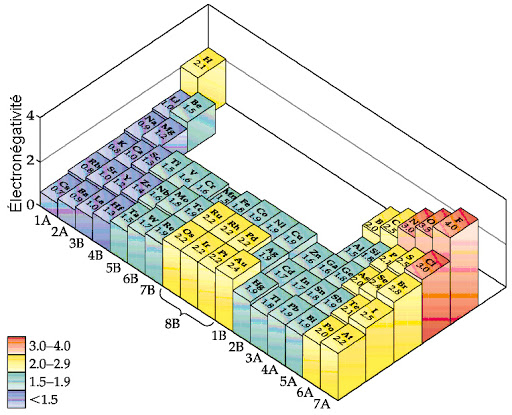
\includegraphics[scale=.6]{chimiePC/atomes/electroneg.jpg}
        \caption{\'Evolution de l'électronégativité au sens de Pauling dans la classification périodique.}
        \label{fig:my_label}
    \end{figure}
\end{EnvUplevel}

\begin{EnvUplevel}
On étudie la réactivité de différents composés organométalliques H$_3$C--M, où M est un atome métallique. Selon l'atome M, la réaction conduit à deux produits \textbf{A} et \textbf{B} en proportion variable comme l'indique la table ci-dessous.

\begin{table}[H]
    \centering
    \begin{tabular}{rlccr}
        Organométallique & H$_3$C--M  & \% ion. C--M & \textbf{A} : \textbf{B} \\ \hline\hline
        Organopotassique      & H$_3$C--K    & 53 & $\sim 1:0$~ \\
        Organosodique         & H$_3$C--Na   & 48 & $99:1$~ \\
        Organolithien         & H$_3$C--Li   & 46 & $98:2$~ \\
        Organomagnésien mixte & H$_3$C--MgBr & 32 & $86:14$ \\
        Organozincique mixte  & H$_3$C--ZnBr & 32 & $72:28$ \\
        Organocuprate lithié  & H$_3$C--CuLi & 10 & $\sim 0:1$~ \\ \hline
    \end{tabular}
    \caption{Propriétés et sélectivité de différents composés organométalliques.}
\end{table}
\end{EnvUplevel}

\question Que signifie l'appellation 'atome métallique' ? Cette appellation est-elle propre ? Décrire quels atomes de la classification périodique peuvent être qualifiés de métalliques.

\question Expliquer l'évolution du pourcentage d'ionicité de la liaison C--M dans la table ci-dessus.

\question Justifier que la réactivité de H$_3$C--M est conditionnée par l'ionicité de la liaison C--M. \\
Réécrire H$_3$C--M dans la limite d'un comportement 100 \% ionique.

\question Donner rapidement la configuration électronique de valence des atomes métalliques K, Na, Li, Mg, Zn, Cu et Mg. \\
On utilisera les abréviation [He], [Ar] et [Ne] (resp. 1$^\text{ère}$, 2$^\text{ème}$ et 3$^\text{ème}$ période).

\question À l'aide de la question précédente, justifier la forme des composés organométalliques (qui sont quasi-ioniques) dans la table ci-dessus.

\question Définir et décrire l'évolution du potentiel d'ionisation dans la table périodique.

\question Les organométalliques H$_3$C--M réagissent très bien avec H$_3$C--Br. Justifier susccintement.

\question Décrire et commenter succinctement l'évolution de la proportion \textbf{A} : \textbf{B}.

\question Qu'en-est-il du rayon ionique de M ?

\end{questions}

\end{exercise}